\section{Materials and Methods} \label{section:materialsAndMethods}
In this section the transformation of the logging data received from e-Vita to the \code{.arff} format of Weka is described. Also, the way in which we determined the attributes and defined adherence is elaborated on.
\subsection{Given data} \label{subsection:givenData}
The provided data is an Excel file with four columns and 9415 rows. The columns contain the \emph{ResearchNumber}, \emph{DateTimeTag}, \code{Code} and \code{ExtraInformation}. Each row represents one action performed by a specific user on the e-Vita website. The research number is a unique identifier per user, providing the ability to group the data per user. The code column denotes which action the user executed, as described in Table~\ref{table:codes}. The extra information field yields information about the section that the user visited, the type of measurement that occurred, or an actual measurement value.

\begin{table}[!h]
	\centering
	\caption{Used codes in the data, and their count}
	\label{table:codes}
	\begin{tabular}{@{}lll@{}}
		\toprule
		\textbf{Code} & \textbf{Description}                                                                              & \textbf{Count} \\ \midrule
		10            & Homepage                                                                                          & 3314           \\
		21            & Opening lab values                                                                                & 391            \\
		22            & Clicking explanation of certain lab value                                                         & 1702           \\
		30            & Opening monitoring                                                                                & 184            \\
		31            & Opening graph of certain measurement                                                              & 231            \\
		33            & Opening graph previous measurements                                                               & 79             \\
		34            & Opening target values                                                                             & 69             \\
		35            & Adding new measurement                                                                            & 162            \\
		40            & Clicking button for extra information                                                             & 477            \\
		50            & Opening coaching                                                                                  & 448            \\
		51            & Clicking button “New wish”                                                                        & 53             \\
		52            & Adding new wish                                                                                   & 26             \\
		53            & Clicking button “Choose goals”                                                                    & 50             \\
		54            & Adding new goal                                                                                   & 35             \\
		55            & Change goal status                                                                                & 5              \\
		56            & Adding new action                                                                                 & 22             \\
		57            & Click button “Evaluate action”                                                                    & 12             \\
		58            & Adding new evaluation                                                                             & 9              \\
		59            & Click button “Ask for coaching”                                                                   & 12             \\
		60            & \begin{tabular}[c]{@{}l@{}}Click button “Yes, the response of the \\ coach is clear”\end{tabular} & 8              \\
		70            & Opening function for extra information                                                            & 401            \\
		71            & Actual opening the extra information                                                              & 235            \\
		90            & Opening function for education                                                                    & 630            \\
		91            & Actual opening education modules                                                                  & 859            \\ \bottomrule
	\end{tabular}
\end{table}

To process the given data, it first was saved as a tab separated file from Excel. Then a Java program reads this file and executes a couple of steps to get the data structured in a way that is easy to process by Weka. The following list shows the steps that were executed.

\begin{enumerate}
	\item Read the tab separated file.
	\item Go through the tab separated file line by line, create an Action object for each line. An Action contains the user id, date, code and extra information fields. The Action object is added to a map that maps user ids to a set with their actions, in Java this is represented by the following structure:\\ \code{Map< String, SortedSet<Action> >}. The Action object of a user are sorted by date to make the next step easier.
	\item Group the list of actions for a user into Session objects. A Session object holds the user id and a SortedSet of Actions. This involves going through the Actions of a user, and adding them to a Session while the time between them is 30 minutes or less. If there is more time in between then it starts a new session. This will output the following data structure:\\ \code{Map< String, SortedSet<Session> >}. The Session objects are sorted by date, so that the first Session of a user is at the start.
\end{enumerate}

\begin{table}[!h]
	\centering
	\caption{Basic statistics of the provided data}
	\label{table:dataStats}
	\begin{tabular}{@{}ll@{}}
		\toprule
		Users                       & 301   \\
		Actions                     & 9414  \\
		Actions per user (average)  & 31.28 \\
		Sessions                    & 1187  \\
		Sessions per user (average) & 3.94  \\ \bottomrule
	\end{tabular}
\end{table}

The described process will deliver an in-memory representation of the data, which helps to detect adherence and determine attributes later. A couple of statistics about the data after processing this step can be found in Table~\ref{table:dataStats}. The exact code used for processing the files can be found on GitHub\footnote{https://github.com/NLthijs48/eVita}. A representation of the data layout can be seen in Figure \ref{figure:dataLayout}.

\begin{figure}[!h]
	\centering
	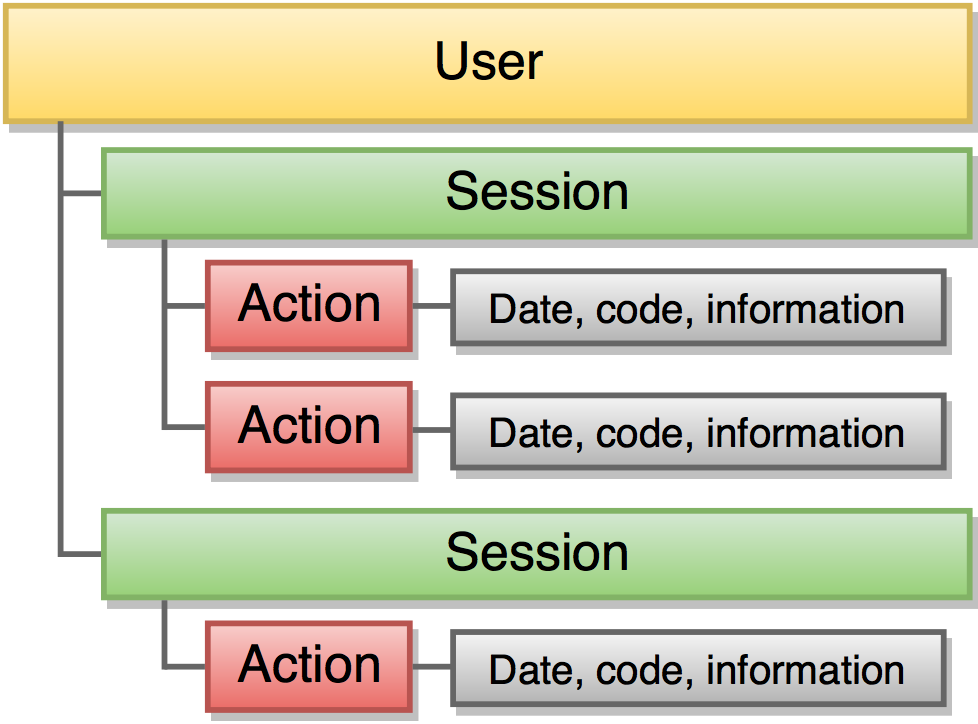
\includegraphics[width=80mm]{dataSmall.png}
	\caption{In-memory data layout}
	\label{figure:dataLayout}
\end{figure}

Since the adherence attributes will use the code fields quite often, some exploration has been done on the presence of each code in the data set. In Table~\ref{table: codes} the number of times a code is used in an action is listed.

\subsection{Adherence definition}
Adherence in the context of the e-Vita website means that the user interacts with the website in a way that we think the user is actually using the website for something, instead of just trying it once. This is a property of the user that we are trying to predict based on the behaviour of the user in the first session. For this process we first need to determine which users are actually adhered and which are not. The definition of adherence is given below, if any of the given conditions is true, then we consider the user to be adherent.

\begin{itemize}
	\item The user visits the application four times or more a year.
	\item The user added at least one personal, health-related goal (code 52).
	\item The user has followed at least one education module (code 91).
	\item The user added measurements (code 35) on four different days.
\end{itemize}

The requirement of logging in at least four times a year is translated as follows: The number of sessions of a user needs to be at least once each 3 months between his first and last login. This means that a user that logged in twice in the period of two months meets the requirement. But a user that logged in twice in seven months, does not meet the requirement. The translation for this requirements is needed since it is a data set of only one year, so for a good prediction, we need to focus on smaller time frames within a year.

\subsection{Attributes} \label{subsection:attributes}
To give input to the classifiers of the Weka tool, we need to define attributes and determine the values for them per user. Since we want to predict the adherence based on the first session of the user, the attributes will only use the data of the first session as input. Below, the different attributes are explained.

\subsubsection{Code frequency attribute}
The first attribute counts the number of times a certain code occurs during the first session. For example, if you give it the code \code{35} in the constructor, then it will count the number of times the user has added a new measurement (listed in Table \ref{table:codes}) in the first session of using e-Vita. This attribute has been generated for all codes listed in Table \ref{table:codes}. Since using certain attributes might predict that the user will be adherent, these attributes are considered more valuable.

\subsubsection{Actions in the first session}
This attribute counts the number of actions the user performed in its first session. The number of actions in the first session could say something about how interested the user is, and might, therefore, predict the adherence.

\subsubsection{Session length}
The session length attribute counts how many minutes the user used e-Vita in his first session. For this, the same applies as for the actions attribute, it might indicate that the user is more interested in the application if he spends more time.

\subsubsection{Actions per hour}
This attribute combines the last two attributes and defines the actions per hour the user performed in his first session.

\subsubsection{Days between sessions}
Two more attributes were added; the number of days between the first and second session, and the number of days between the second and third session. These attributes do not purely use data from the first session but were independently used to predict the adherence of a user instead of the other attributes.

\subsection{Creating a Weka file}
As input the Weka tool requires an \code{.arff} file. This is a simple file format where you first define the columns and then provide the data\footnote{http://www.cs.waikato.ac.nz/ml/weka/arff.html}. Using the structured data from Section \ref{subsection:givenData} and the attributes from Section~\ref{subsection:attributes} this file for Weka was generated.

\subsection{Using Weka} \label{subsection:usingWeka}
Based on the research questions a couple of different things were analysed. The following sections describe the different techniques that were used.

\subsubsection{Predictors of adherence: First session}
For this analysis, all attributes that only use data of the first session were used. That means the 'days between sessions' attributes were discarded. First, we ranked the attributes on their information gain, for this the \code{InfoGainAttributeEval} attribute evaluator plus the \code{Ranker} search met\allowbreak hod have been used. This produces a list of the most important attributes. After this a classification was performed with the \code{ADTree} classifier (using cross-validation, 10 folds). This results in a performance score, confusion matrix, and a decision tree. A decision tree classifier was applied to give a good impression of the decision process. It can easily be compared to the ranking of the attributes and can easily be checked for correctness. If for example the top node of the tree would be an attribute like visiting the home page, then this might indicate something is wrong.

\subsubsection{Predictors of adherence: Days between sessions}
This analysis only uses the attributes that describe the number of days between sessions as input. Again the \code{InfoGainAttributeEval} attribute evaluator plus the \code{Ranker} search method have been used to rank the attributes. After this, the \code{BFTree} classifier has been used. The classifier produced the confusion matrix and decision tree.

\subsubsection{Prediction of days between sessions}
The next question to answer is if we can predict the number of days between sessions one and two, and between sessions two and three, using the attributes of the first session. For this, the \code{LinearRegression} algorithm was utilized (with cross-validation, 10 folds). This regression algorithm tries to calculate a formula with which the number of days between the sessions can be calculated, based on the attributes. The algorithm shows performance results such as the correlation coefficient, mean absolute error, root mean squared error, relative absolute error and root relative absolute error. Because the number of days between the first and second session is not known for all users, since some do not have a second session yet, Weka will ignore those instances (a \code{?} is passed as value for the attribute, which means a missing value in the \code{.arff} format). The number of ignored instances will be higher for the days between the second and third session since even fewer users have a third session.










